 \newif\ifpdfmadness

\ifx\pdfoutput\undefined
   \pdfmadnessfalse
\else
   \ifnum\pdfoutput=1
     \pdfmadnesstrue
   \else
     \pdfmadnessfalse
   \fi
\fi

\documentclass[preprint,nonatbib,blockstyle,nocopyrightspace,times]{sigplanconf}

\newcommand\txprobj[3][]{a#1_{#2_{j-1}#3_j}}
\newcommand\txprobjj[3][]{a#1_{#2_{j-1}#3_j}}
\newcommand\alignwidth{\ensuremath R} % number of columns in an alignment
\newcommand\pairedwith[1]{{\pi(#1)}}

\newcommand\naive{na\"\i ve}
\usepackage{amsmath}
\usepackage{array}
\usepackage{listings}
\usepackage{graphicx}
\lstset{
    tabsize = 2,
    basicstyle = \ttfamily,
    language = Haskell
    }    

\newcommand\figref[1]{Figure~\ref{#1}}
\newcommand\secref[1]{Section~\ref{sec:#1}}
\newcommand\seclabel[1]{\label{sec:#1}}

\usepackage{verbatim}

\newenvironment{smallverbatim}{\par\small\verbatim}{\endverbatim}
\newcommand\smallverbatiminput[1]{{\par\unskip\small\verbatiminput{#1}}}
\newcommand\smallfuzzverbatiminput[2]{{\par\unskip\small\hfuzz=#1 \verbatiminput{#2}}}

\renewcommand\ttdefault{aett}

  \long\def\remark#1{%
      \ifvmode
         \marginpar{\raggedright\hbadness=10000
         \parindent=8pt \parskip=2pt
         \def\baselinestretch{0.8}\tiny
         \itshape\noindent #1\par}%
      \else
          \unskip\raisebox{-3.5pt}{\rlap{$\scriptstyle\diamond$}}%
          \marginpar{\raggedright\hbadness=10000
         \parindent=8pt \parskip=2pt
         \def\baselinestretch{0.8}\tiny
         \itshape\noindent #1\par}%
      \fi}

\usepackage[authoryear]{natbib}
\bibpunct();A{},
\let\cite\citep
\let\citeyearnopar=\citeyear
\let\citeyear=\citeyearpar


\begin{document}


\conferenceinfo{ICFP '12}{September 9-15, Copenhagen.} 
\copyrightyear{2012} 
\copyrightdata{[to be supplied]} 

%\titlebanner{banner above paper title}        % These are ignored unless
\preprintfooter{Haskell in Computational Biology}   % 'preprint' option specified.

\title{Experience Report: Haskell in Computational Biology}
% \subtitle{Subtitle Text, if any}

\authorinfo{Noah M. Daniels \and Andrew Gallant \and Norman Ramsey}
           {Department of Computer Science, Tufts University}
           {\{ndaniels, agallant, nr\}@cs.tufts.edu}


\maketitle

\begin{abstract}
In computational biology, the languages of choice for solving ad-hoc problems are high-level
``scripting'' languages such as Python or domain-specific statistics languages such as R,
while the language of choice for solving high-performance problems is C++.
This dichotomy creates a difficulty when computational biologists wish to experiment with a
variety of approaches to a problem, only some of which are likely to prove fruitful.
This experience report details our use of Haskell in implementing a high-performance,
computational biology application which is the first implementation of a particular
novel algorithm for protein structure and function prediction. We discuss the highlights
and difficulties of this project, as well as the potential improvements the Haskell
community might make that would ease some of these difficulties.
\end{abstract}

% \category{CR-number}{subcategory}{third-level}
% 
% \terms
% term1, term2
% 
% \keywords
% keyword1, keyword2

\section{Introduction}

Computational biologists write software that answers questions about 
sequences of nucleic acids (genomic data) or sequences of amino 
acids (proteomic data). 
For some software, considerations of performance are paramount; this
software is usually written in C~or~C++. 
For other software, considerations of convenience, readability, and
productivity are more important;
this software is usually written in a high-level, dynamically-typed
``scripting'' or domain-specific language like
Perl, Python, Ruby, SPSS, or~R.\remark{Don't forget audience.}
In~this Experience Report, we show that computational biologists can
successfully replace both these families of languages with Haskell:
\begin{itemize}
\item
Our experimental Haskell programs are as easy to understand and change
 as the programs our group writes using scripting languages.
\item
The performance of our Haskell code is comparable to the performance
of~C++.
\item
Although we have had to write a new implementation of a standard
algorithm, the cost was low, and the connection between code and
algorithm is unusually strong (\secref{viterbi}).
\item
We have experienced barriers to entry, of which the most salient has been
the difficulty of understanding and tuning  the performance of Haskell
programs. 
We found the other barriers 
relatively easy to overcome.
\end{itemize}
Our experience is based on MRFy (pronounced ``Murphy''), which
implements a novel family of algorithms for finding remote homologs to 
newly discovered proteins. 

\emph{[Alternate introduction, trying to tie the points more closely
to the content of the paper:\\
In~this paper, we report on an attempt to replace both these families
of languages with Haskell: 
\begin{itemize}
\item
Although had to write a new implementation of a standard
algorithm, the cost was low, and the connection between code and
algorithm is unusually strong (\secref{viterbi}).
The performance of our new implementation is comparable to the
performance of~C++.
\item
As expected, higher-order functions made it unusually easy to
implement and experiment with a family of related algorithms
(\secref{hofs}).
\item
Haskell is surrounded by a penumbra of libraries and tools that
promise powerful abstractions.
Some deliver very high leverage, but others are not ready for prime
time (\secref{penumbra}).
We~found it difficult to tell which is which in advance.
\item
It is possible to use Haskell successfully for research even with a
very modest background in functional programming. 
\item
The only significant impediment that Haskell pas presented to our
research has been the difficulty of understanding and tuning the
performance of Haskell programs.
\end{itemize}
]}



\section{The biology}

Proteins are cellular machinery. They interact with one another and with other 
molecules to carry out the functions of living cells: metabolism, regulation, 
signalling, and more.
A~protein's function is determined by its structure, 
and its structure is determined by the sequence of amino acids that
form the protein.
\remark{Lost: there are only 20-odd amino acids}
The amino-acid sequence is ultimately determined by a sequence of
nucleic acids in DNA, which we call a gene.
Given a genetic sequence, biologists wish to know the cellular
function of the protein that gene codes for.
The best known method of discovering such function is
to find other proteins of 
similar structure, which likely share similar function.
Proteins that share structure and function are expected to be
descended from a common ancestor---in biological terms, \emph{homologous}---and
thus
the problem of identifying proteins similar to a \textit{query sequence} is called 
\textit{homology detection}.




Computational biologists detect homologies by building 
algorithms which, given a \emph{query sequence} of amino acids,
find known proteins of similar structure.
When the similar proteins are formed from amino-acid sequences that
are not too different from the query sequence, the homology can be
detected by
a family of algorithms called 
\textit{hidden Markov models}~\cite{Eddy:1998ut}.
But in real biological systems,
proteins with similar structure and function may be formed from significantly 
different amino-acid sequences, which are not close in edit distance.
Our~research contribution---the MRFy algorithm---can detect homologies
in amino-acid sequences that are only distantly related.
%
%We will explain an 
%algorithm for detecting reasonably similar sequences, and then move on to 
%explain MRFy, our novel approach for detecting more distantly related sequences 
%for proteins that share similar structure and function.
%
To~enable you to understand our experience with Haskell,
we~sketch not only the MRFy algorithm (\secref{mrfy})
but also one of the older hidden-Markov algorithms (\secref{viterbi}),
which is incorporated into~MRFy.

\remark{LOST: We conclude that implementations of mathematically-intensive 
algorithms such as these lend themselves to the Haskell language, particularly 
when the programmer needs a flexible implementation that simplifies 
experimenting with variants of the algorithm.}


% As a brief refresher in the standard dogma of genetics, recall that genes 
% (strands of deoxyribonucleic acid (DNA), which are sequences of the nucleotides 
% adenosine, cytosine, guanine, and thymine, represented by the letters A, C, G, 
% and T) are transcribed into ribonucleic acid (RNA). Some RNA is then translated 
% into the 20 naturally-occuring amino acids, which form peptide chains -- 
% proteins -- which fold into complex structures in the cell. These proteins are 
% cellular machinery, performing the varied functions an organism needs to 
% survive. 

% However, determining what newly sequenced genes actually do -- when they become 
% proteins, what structures those proteins fold into, and what functions they 
% perform -- has not kept pace. Determining the atomic coordinates of a newly 
% discovered protein may require as much as two graduate-student-years in a lab! 
% Fortunately, determining the full structure of a protein is not always 
% necessary. Often, we can identify well-known proteins of similar sequence or 
% structure to a new protein, and thus make educated guesses as to the structure 
% and function of the new protein.
% 
% The problem of taking a newly found protein sequence about which only the 
% sequence is known, and determining what existing proteins of known structure 
% and function most closely resemble that new protein, is known as homology 
% detection. When proteins of similar sequence can be found, this problem is 
% largely solved. To solve the homology detection problem, computational 
% biologists have developed fast, approximate methods for determining the 
% structure and function of proteins based on their sequence. The most popular 
% software for homology detection is called HMMER, which uses a hidden Markov 
% model to capture evolutionary change.

% However, when there are no known proteins of similar sequence, only 
% evolutionarily distant proteins that may share similar structure, this problem 
% is called remote homology detection. Hidden Markov model approaches begin to 
% fail as sequence similarity falls off. Recently, Markov random field 
% approaches, which capture non-local interactions in the protein structure, have 
% been shown to perform well. However, these approaches face the challenge of 
% increased computational complexity; the SMURF program exhibits exponential time 
% complexity, while SMURFLite (work by one of the authors) bounds the exponent by 
% simplifying the Markov random field's dependency graph. MRFy is a 
% stochastic search approach to Markov random fields.

\section{The Software}

%% \subsection{The Viterbi Algorithm}

\seclabel{viterbi}

Homology-detection software is most often used in one of two ways:
to test a hypothesis about 
the function of a single, newly discovered protein, or 
to compare every protein in a genome against a library of known protein 
structures.
Either way, 
the software is \emph{trained}
on a group of proteins that share function and structure.
These proteins are identified by a biologist, who puts
their amino-acid sequences into a correspondence, also called an
\emph{alignment}. 
This alignment represents structural
correspondence among individual amino acids in a set of homologous proteins.
An~alignment may be represented as a matrix
(Figure~\ref{alignment}) 
in which each row corresponds to the amino-acid sequence of a protein,
and each column groups amino acids that play similar roles in
different proteins.


An alignment may contain \emph{gaps} (notated as dashes in
\figref{alignment}) for some proteins.
A~gap in row~2, column~$j$ indicates that as proteins evolved, either 
protein~2 lost its amino acid in position~$j$, or 
other proteins gained an amino acid in position~$j$.
If~column~$j$ contains few gaps, 
it~is considered a \emph{consensus column},
and the few proteins with gaps probably lost amino acids via
\emph{deletions}.\remark{NMD: Missing is the fact that all these models
are directionless; they don't care whether something was gained or lost
over time. Perhaps this doesn't matter.}
If~column~$j$ contains \emph{mostly} gaps, 
it~is considered a \emph{non-consensus column},
and the few proteins without gaps probably gained amino acids via
\emph{insertions}. 

Once a protein alignment is constructed, it~is used to train a
\emph{hidden Markov model}. 
A~hidden Markov model is a probabilistic finite-state machine which 
can assign a probability to any query sequence.
A~protein whose query sequence has a higher probability is more likely to %
be homologous to the proteins in the alignment.
We~write a query sequence as $x_1, \ldots, x_{\scriptscriptstyle N}$,
where each $x_i$~is 
an amino acid.
$N$~need not be the same as the number of columns in the alignment,
which we write~\alignwidth.


\begin{figure}
\ifpdfmadness
\centerline{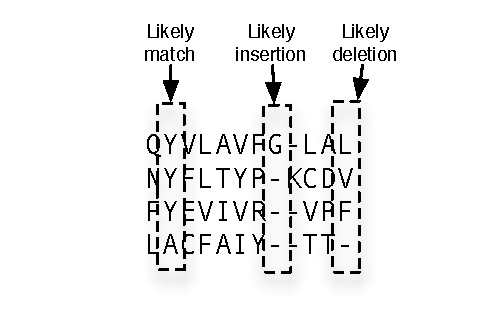
\includegraphics[width=6cm]{alignment.pdf}} 
\else
\centerline{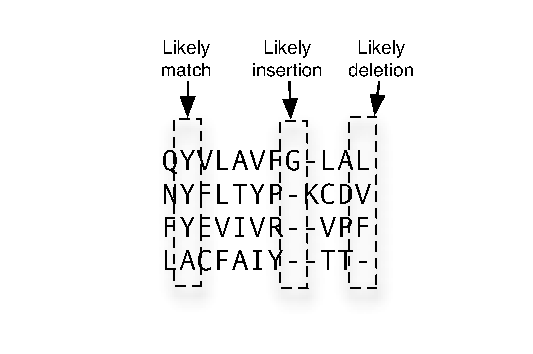
\includegraphics[width=6cm]{alignment.eps}} 
\fi



\caption{A~structural alignment of four proteins $(\alignwidth = 4)$}
\label{alignment} 
\end{figure}

A~hidden Markov model carries probabilities on its states and on its
state transitions.
Both the probabilities and the
the states are determined by the alignment:
\begin{itemize}
\item
For each column~$j$ of the alignment, the hidden Markov model has a
\emph{match state}~$M_j$.
The match state contains a table $e_{M_j}(x)$ which gives the
 probability that a homologous protein has amino acid~$x$ in
 column~$j$.
This probability is called an \emph{emission} probability.
\item
For each column~$j$ of the alignment, the hidden Markov model has a
\emph{deletion state}~$D_j$.
The deletion state determines the probability that the query sequence
has \emph{no} amino acid  in column~$j$, i.e., that it has a gap.
\item 
For each column~$j$ of the alignment, the hidden Markov model has an
\emph{insertion state}~$I_j$.
The insertion state contains a table $e_{I_j}(x)$ which gives the
probability that a homologous protein has gained amino acid~$x$ by
insertion at column~$j$.
\end{itemize}
The hidden Markov model also has distinguished \emph{begin} and \emph{end} states.

The particular hidden Markov model we use requires that every nonempty
sequence of insertions be followed by a match, and similarly for
deletions.
\remark{citation needed?}
In~other words, insertions and deletions cannot be mixed without an
intervening match.
This restriction means that between two adjacent columns, six
transitions are possible.
An~insertion state may also transition to itself.
\begin{itemize} 
\item
A~transition into a match state in
column~$j$ is more likely when column~$j$ is a consensus column.
Depending on the predecessor state, 
the probability of such a transition is notated
$\txprobj M M$, $\txprobj I M$, or $\txprobj D M$.
\item
A~transition into a deletion state in
 column~$j$ is more likely when column~$j$ is a non-consensus column.
The probability of such a transition is notated
$\txprobj M D$ or $\txprobj D D$.
\item
A~transition into an insertion state in
 column~$j$ is relatively unlikely,
but it is more likely when column~$j$ is a non-consensus column.
The probability of such a transition is notated
$\txprobjj M I$ or $\txprobjj I I$.
\end{itemize}



\begin{figure} 
\ifpdfmadness
\centerline{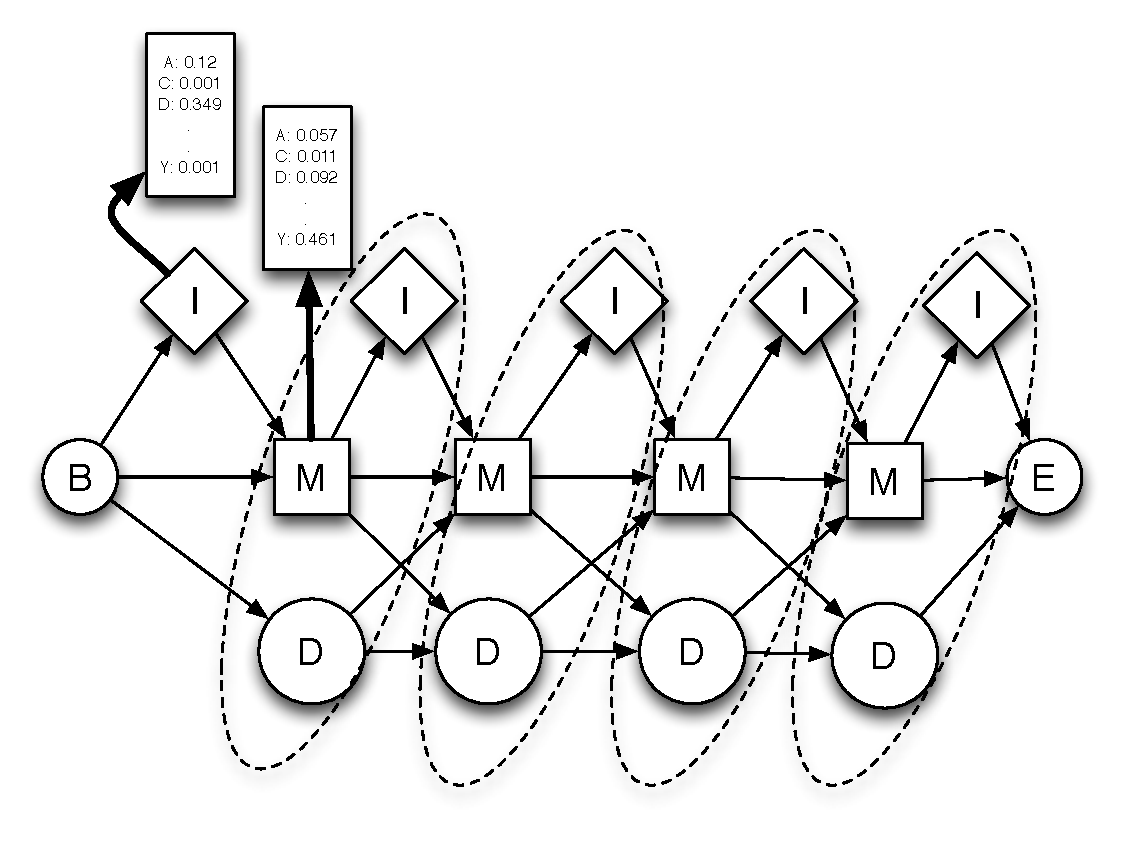
\includegraphics[width=8cm]{Plan7.pdf}} 
\else
\centerline{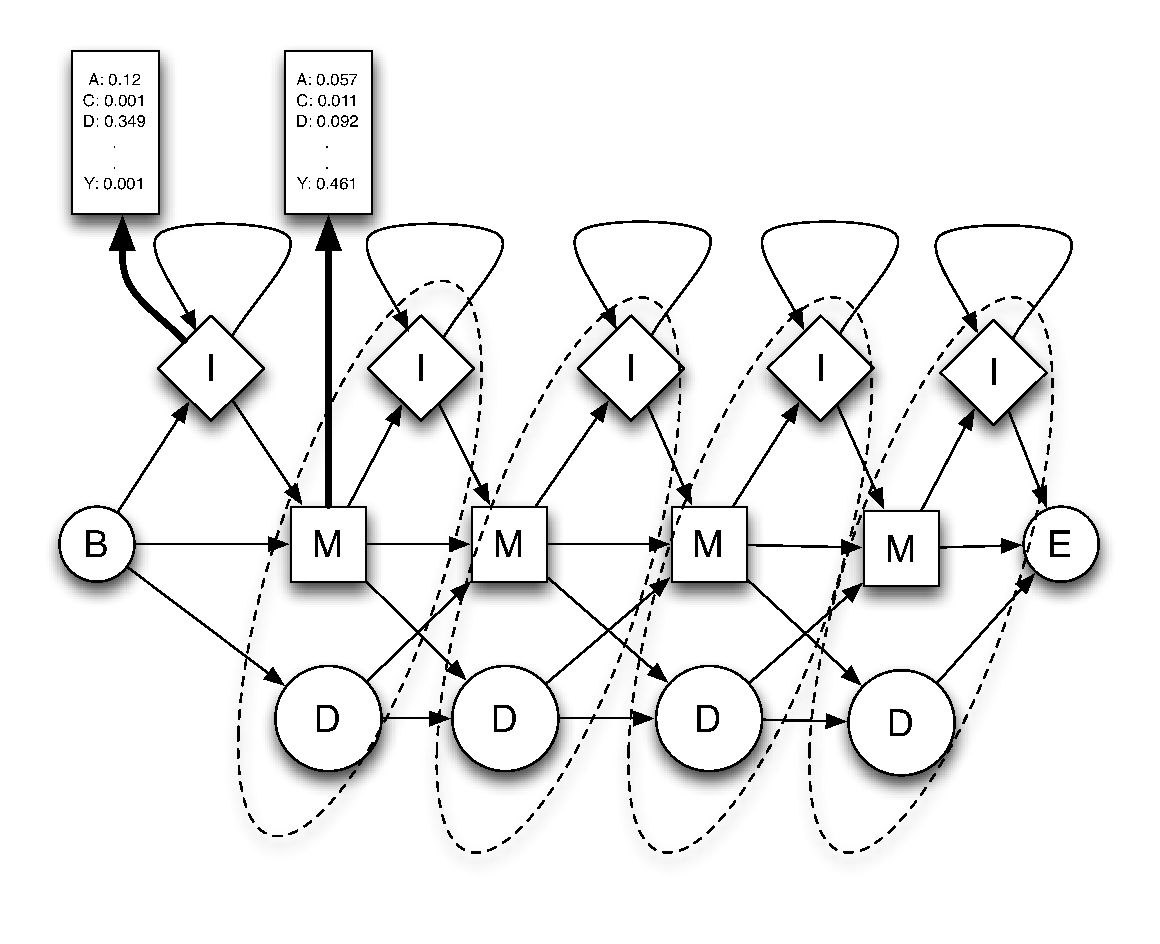
\includegraphics[width=8cm]{Plan7.eps}} 
\fi


This model
has begin and end states $B$~and~$E$,
as well as four
nodes, each containing 
an insertion state~$I$, 
a match state~$M$, and a
deletion state~$D$.

\caption{A hidden Markov model $(\alignwidth = 4)$}

\label{plan7} \end{figure}



\begin{figure*}
\def\goo{18pt}
\def\gum{14pt}
\[
\begin{array}{l@{}c@{}l}
V_{j}^{M}(i) &{}={}& \log\frac{e_{M_{j}}(x_{i})}{q_{x_{i}}} + \max \left\{
\begin{array}{l l}
V_{j-1}^{M}(i - 1) + \log a_{M_{j-1}M_{j}}\\
V_{j-1}^{I}(i - 1) + \log a_{I_{j-1}M_{j}}\\
V_{j-1}^{D}(i - 1) + \log a_{D_{j-1}M_{j}}\\
\end{array} \right.\\[\goo]
V_{j}^{I}(i) &=& \log\frac{e_{I_{j}}(x_{i})}{q_{x_{i}}} + \max \left\{
\begin{array}{l l}
V_{j}^{M}(i - 1) + \log a_{M_{j}I_{j}}\\
V_{j}^{I}(i - 1) + \log a_{I_{j}I_{j}}\\
\end{array} \right.\\[\gum]
V_{j}^{D}(i) &=& \max \left\{
\begin{array}{l l}
V_{j-1}^{M}(i) + \log a_{M_{j-1}D_{j}}\\
V_{j-1}^{D}(i) + \log a_{D_{j-1}D_{j}}\\
\end{array} \right.\\
\end{array}
\qquad
\begin{array}{l@{}c@{}l}
V_{j}^{\prime M}(i) &{}={}& e^{\prime}_{M_{j}}(x_{i}) + \min \left\{
\begin{array}{l l}
V_{j-1}^{\prime M}(i - 1) + a^{\prime}_{M_{j-1}M_{j}}\\
V_{j-1}^{\prime I}(i - 1) + a^{\prime}_{I_{j-1}M_{j}}\\
V_{j-1}^{\prime D}(i - 1) + a^{\prime}_{D_{j-1}M_{j}}\\
\end{array} \right.\\[\goo]
V_{j}^{\prime I}(i) &=& e^{\prime}_{I_{j}}(x_{i}) + \min \left\{
\begin{array}{l l}
V_{j}^{\prime M}(i - 1) + a^{\prime}_{M_{j}I_{j}}\\
V_{j}^{\prime I}(i - 1) + a^{\prime}_{I_{j}I_{j}}\\
\end{array} \right.\\[\gum]
V_{j}^{\prime D}(i) &=& \min \left\{
\begin{array}{l l}
V_{j-1}^{\prime M}(i) + a^{\prime}_{M_{j-1}D_{j}}\\
V_{j-1}^{\prime D}(i) + a^{\prime}_{D_{j-1}D_{j}}\\
\end{array} \right.\\[\gum]
\multicolumn3{l}{%
a'_{s} = - \log a_{s} 
\qquad
e^{\prime}_{s,x} = - \log\frac{e_{s,x}}{q_{x}}
\qquad
V_j^{\prime M}(i) = - V_j^{M}(i)
}
\\
\end{array}
\]

\caption{Viterbi's equations, in original and negated forms}
\label{viterbi}
\end{figure*}



\subsection{Computing probabilities using perspicuous Haskell}

Given a hidden Markov model, 
an~established software package called HMMER (``hammer'') 
can compute the probability
that a new protein shares structure and
evolutionary history with the proteins used to train the model.
The computation finds the most likely path through the hidden Markov model.
To~make best use of floating-point arithmetic, the software computes
the \emph{logarithm} of the probability of each path, by summing
the logs of the 
probabilities on the states and edges of the path \cite{Viterbi:1967hq}.
(The logarithm function is monotonic, so the path that maximizes the
log of the probability is the most likely path.)
The~specification is shown on the left-hand side of \figref{viterbi}.
The probability $V_j^M(i)$ represents the probability of the most
likely path of the first~$i$ amino acids in the query sequence,
terminating with placement of amino acid $x_i$ in state~$M_j$.
The probabilities $V_j^D(i)$ and $V_j^D(i)$ are similar.
Equations like these can be found in more recent literature
\cite{Durbin:1998wz,Eddy:1998ut}. 


To~be able to use Haskell, we had to reimplement the standard
algorithm for solving Viterbi's equations.
Haskell made it possible for us to write code that looks like the
math,
which made the code easy to write and gives us confidence that it is
correct.
We~begin with our representations.

In~idiomatic Haskell, 
we might represent an individual amino acid~$x$
using a value of algebraic data type, thus:
\begin{smallverbatim}
data Amino = Ala | Cys | Asp | Glu | Gly | ...
\end{smallverbatim}
But our primary goal was to get something working quickly with a
legacy file format that represents each amino acid as a small integer.
Our representation is therefore
\begin{smallverbatim}
type AA       = Int -- amino acid using HMMER coding
\end{smallverbatim}
Either way, a query sequence is (and should be) an immutable vector of
amino acids.
%type QuerySeq = Vector AA
%\end{smallverbatim}

The log of a probability is simply a number.
To distinguish a transition probability from other numbers, we wrap it in
the value constructor \texttt{TProb}:
\begin{smallverbatim}
type LogProb = Double
data TProb   = TProb { logProbability :: LogProb }
\end{smallverbatim}
We group transition probabilities into 7-tuples.
Each tuple corresponds to a ``node'' in the hidden Markov model
(a~dashed ovel in \figref{plan7}), and to a column of the original
alignment.
As~noted above, 
a match state may transition to any state in the successor node;
an insertion state may transition to itself or to its successor match
state;
and
a~deletion may transition to its successor match
state or deletion state.
\begin{smallverbatim}
data TProbs = 
     TProbs { m_m :: TProb, m_i :: TProb, m_d :: TProb
            , i_m :: TProb, i_i :: TProb
            , d_m :: TProb, d_d :: TProb }
\end{smallverbatim}

The representation of a node includes the probabilities of transitions
into the three states of that node, plus the tables
of emission probabilities for the match and insertion states.
\begin{smallverbatim}
type EProbs  = Vector LogProb
data HmmNode = HmmNode { transitions  :: TProbs
                       , matEmissions :: EProbs
                       , insEmissions :: EProbs
                       }
\end{smallverbatim}

In~Viterbi's equations,
the probability in each state is a simple function of the probability
in its predecessor states, 
and all probabilities can be computed by a classic dynamic-programming
algorithm
which starts at the begin state,
computes probabilites in nodes $1$~through~$\alignwidth$ in
succession, and terminates at the end state.
One of us implemented this algorithm, storing the probabilities in an array.
\remark{Why is the number of dimensions 3 and not 2 (indices $i$, $j$,
and what??) and why do we care?}
The cost was
$O(|N|\times|\alignwidth|)$;
in our work, $\alignwidth$~and~$N$ range from several hundred to a few
thousand.



%%  For 
%%  reasons including floating point underflow, the HMMER software (with which we 
%%  maintain file format compatibility) stores all probabilities in a trained HMM 
%%  file as negative natural logs.
%%  Thus, the Viterbi recurrence relations are 
%%  simplified from the form in \ref{viterbi_eqn} to that in \ref{viterbi_log_eqn}, 
%%  and because they are \textit{negative} logs, the problem transforms from 
%%  maximization to minimization.

Another of us was curious to try to code Viterbi's equations
directly as recursive functions.
But like the classic recursive Fibonacci function, Viterbi's functions,
when implemented \naive ly,
perform extraordinarily badly.
But just like the Fibonacci function, Viterbi's functions can be
\emph{memoized}.
To~show the memoized code, we have to confess to a small
transformation of Viterbi's equations.
The logarithms on the left of \figref{viterbi} are computed when the
hidden Markov model is constructed, and the resulting numbers are
stored in a file.
Moreover, to make the file more pleasant to read, the logarithms are
negated.
(The logarithm of a probability is typically negative, and negating
the logarithm eliminates hordes of minus signs from the file.)
We~therefore implement a transformed version of Viterbi's equations,
shown on the right-hand side of \figref{viterbi}, which minimize the
negated log probability for each combination of node~$j$, amino
acid~$x_i$, and state $M_j$, $I_j$, or $D_j$.
Our implementation computes not only the minimum
negated log probability, called a \texttt{Score},
but also the path of states which leads to that most likely outcome. 
Because the cases for all three states are so similar, 
we~show only the code for the match state:
%%%%%%%%%%%%%%%%%%%%%%%%%%%%%%%%%%%%%%%%%%%%%%%%%%%%%%%%
\begin{smallverbatim}
viterbi' :: State -> Int -> Int -> (Score, [State])
viterbi' Mat j i = ( eProb j i + minimum $ [ trans m_m Mat
                                          , trans i_m Ins
                                          , trans d_m Del 
                                          ]
                  , Mat : path )
  where (prevV, path) = viterbi prev (j-1) (i-1)
        trans t prev = prevV + tProb hmm (j-1) t
\end{smallverbatim}
% Similarly, the insertion equation is:
% \begin{verbatim}                    
%   -- consume an observation but not a node
%   | s == ins = let trans t prev =
%                    (score + tProb n t + (eProb n o), ins:path)
%                     where (score, path) = viterbi prev n (o - 1)
%                 in minimum [
%                     trans m_i mat,
%                     trans i_i ins
%                     ]
% \end{verbatim}
% Finally, the deletion equation is:
% \begin{verbatim}                    
%   -- consume a node but not an observation
%   | s == del = let trans t prev = 
%                       (score + tProb (n-1) t, del:path)
%                       where (score, path) = viterbi prev (n - 1) o
%                 in minimum [
%                     trans m_d mat,
%                     trans d_d del
%                     ]
% \end{verbatim}
Programming the algorithm in this form was not only intellectually
satisfying; keeping the code close to the math also helped us find
bugs.
The most memorable bug was that in one of our base cases, 
we~mistakenly returned an empty path of states;
the correct result was a singleton path containing the initial state.
Very quickly after observing a missing state in the output, we were
able to find the faulty case in the code.

Whatever the attractions of the code above, in our work we also
require high performance.
To make the simple recursive code efficient, we used Luke Palmer's
\texttt{Data.Memocombinators} package.
The function \verb+viterbi'+ is unmemoized,
and it makes recursive calls to \verb+viterbi+, which is memoized:
\begin{smallverbatim}
viterbi state j i = 
  Memo.memo3 (Memo.arrayRange (Mat, End)) 
             (Memo.arrayRange (0, numNodes))
             (Memo.arrayRange (0, seqlen)) 
             viterbi' state j i
\end{smallverbatim}
The value
\texttt{numNodes} represents~$\alignwidth$,
and \texttt{seqlen} represents~$N$.\remark{I hope this is right. ---NR}

This memoized recursive code performs just as well as the classic
dynamic-programming code.
And~the short fragment above is the \emph{only} part of the code
devoted to improving performance.
By contrast, standard implementations of the Viterbi algorithm, such as in HMMER,
spend much of their code 
managing dynamic-programming tables.
Haskell enabled us write simple, performant code with little effort.
%
Because the memoized version so faithfully resembles the equations in
\figref{viterbi}, we~retired the classic dynamic-programming version.


\remark{NR doesn't think the bug story is that interesting.}

%%  
%%  
%%  In this, we were grateful for the resemblance 
%%  between the mathematical description of the algorithm and the top-down 
%%  dynamic-programming approach in Haskell, which resulted in perspicuous code.
%%  
%%  


\subsection{Exploring new algorithms using higher-order functions}


%\subsection{MRFy Implementation}

Our implementations of hidden Markov models and Viterbi's algorithm
duplicate existing functionality.
They form just one component of our new tool, MRFy.

A hidden Markov model uses local information about
amino-acid sequences.
But real proteins are three-dimensional,
and when a real protein folds, groups of amino acids
that are far away in the one-dimensional sequence can be
adjacent in three-dimensional space.
We~are studying adjacent groups called \emph{beta strands}, which
can become hydrogen-bonded to each other,
and are effectively ``stuck together.''

A~mutation in a paired beta strand may break the pairing, in which
 case the mutated protein will not fold properly and is unlikely to
 survive natural selection.
But a mutation in a paired beta strand \emph{can} survive if it is
 accompanied by a compensatory mutation in the strand with which it is
 paired. 
The probability of finding amino acid $x_i$ in column~$j$ of an alignment may
 therefore depend on the amino acid in the paired column
 $\pairedwith j$.
This nonlocal interaction changes
Viterbi's equations:
each term $V_{j}^{\prime M}(i)$ becomes
$$W_{j}^{M}(i) = V_{j}^{\prime M}(i) - \log P(x_{i} \mid x_{\pairedwith j}).$$
The distance between columns~$j$ and $\pairedwith j$ can be as small
 as a few columns or as large as a few hundreds of columns.


The approach currently taken in computational biology
is~to model each pair of beta strands not with two hidden Markov
models, 
but with a pair of sequences of match states.
Each of the subsequences \emph{between} paired beta strands is then
modeled with an ordinary hidden Markov model.
The~combined model, as shown in \figref{mrf}, is called a
\textit{Markov random field}. 
Because of nonlocal interactions between paired beta strands, 
the likelihood-maximization for a Markov random field does not
 exhibit optimal substructure, and dynamic
 programming cannot solve it quickly \cite{Menke:2010ti,Daniels:2012}.
The~purpose of MRFy is to explore new methods of \emph{approximating}
maximum likelihood.


\begin{figure}
\ifpdfmadness
\centerline{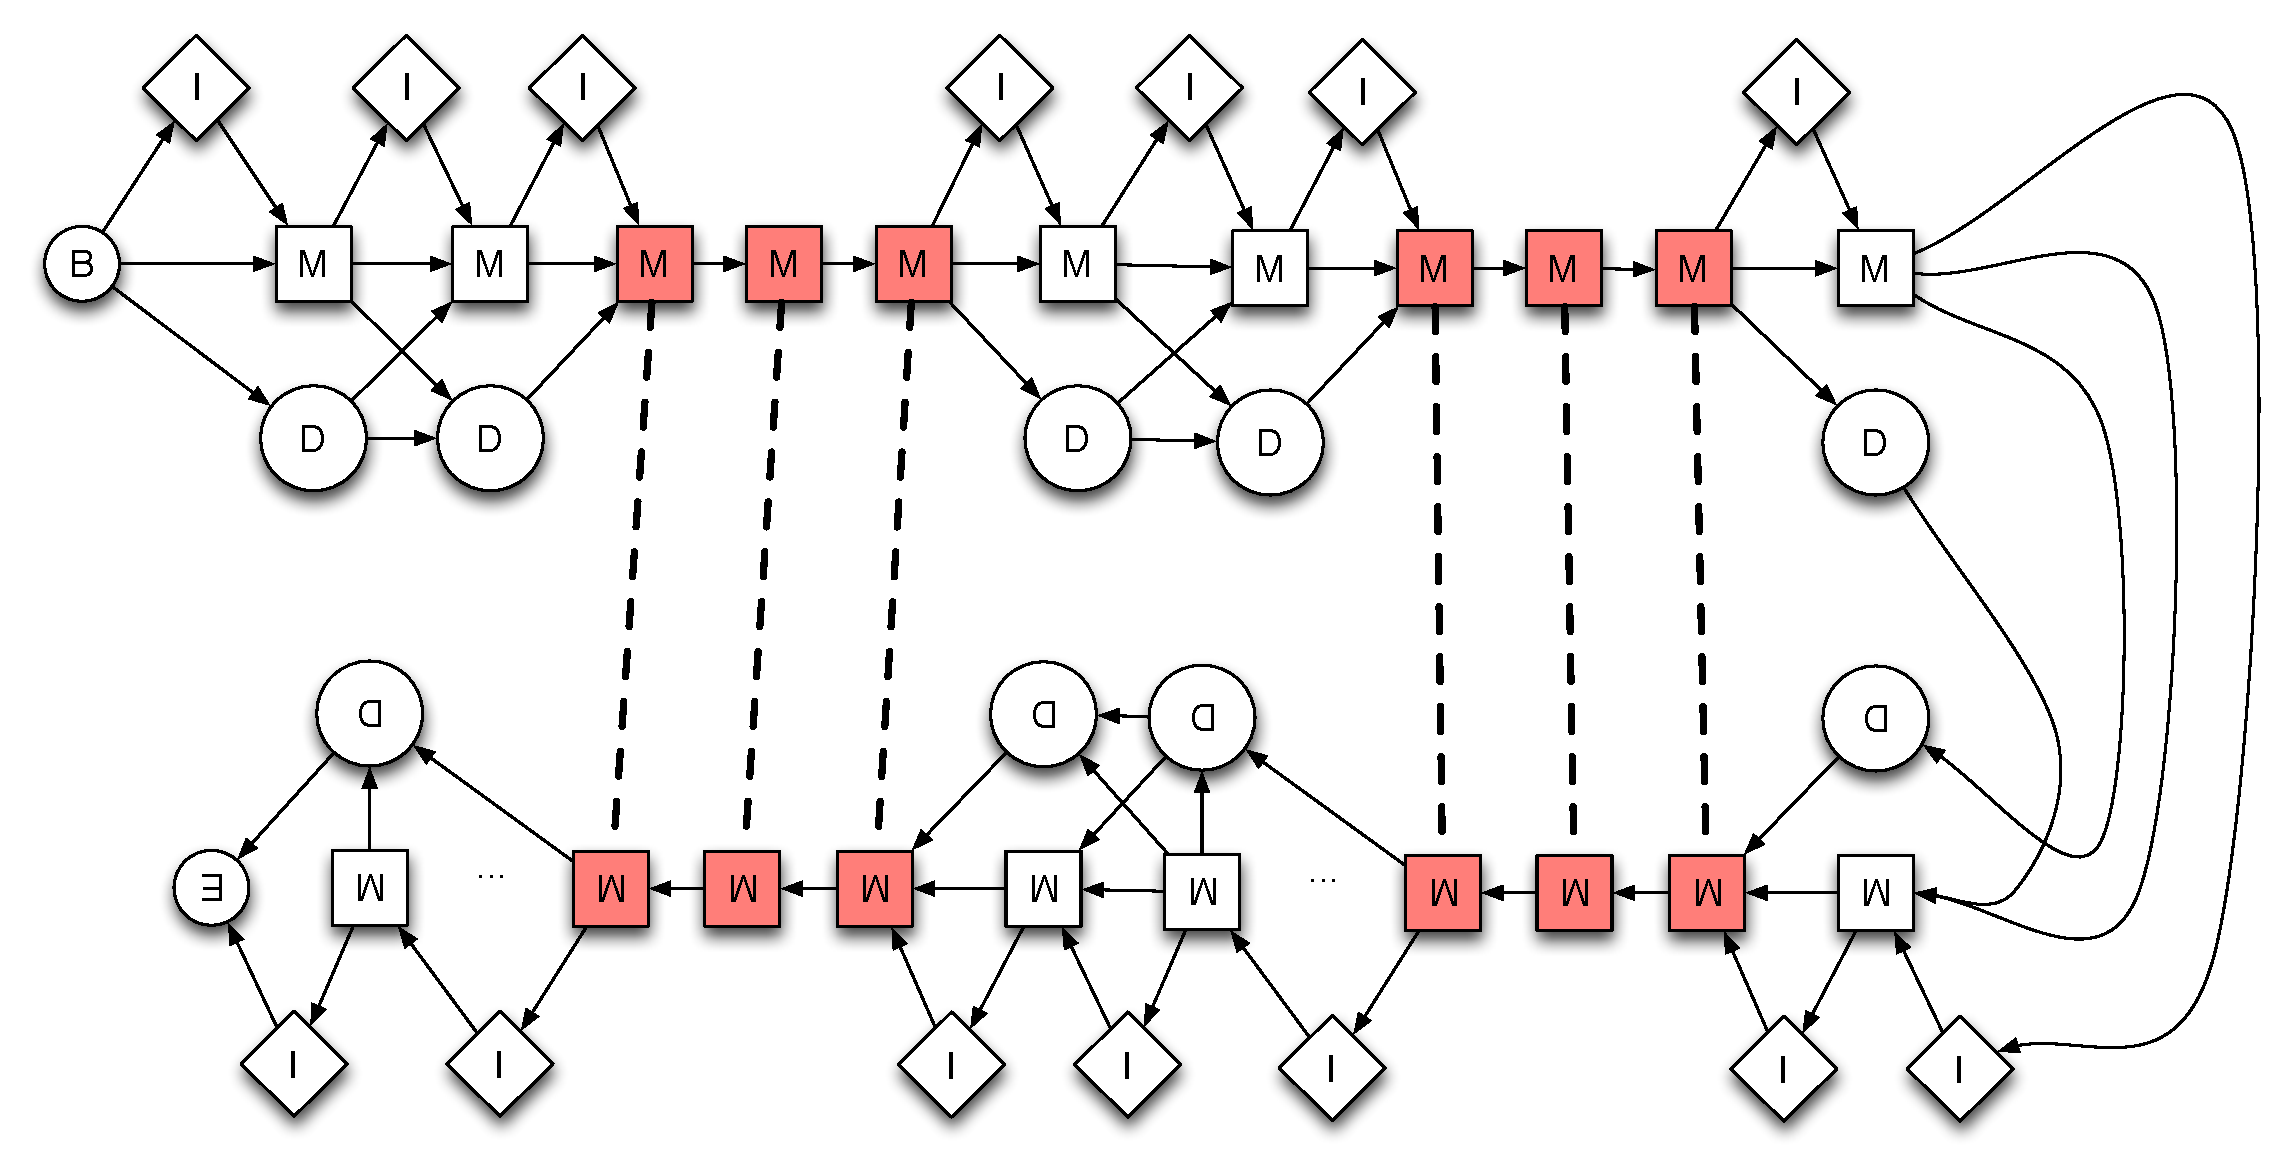
\includegraphics[width=8cm]{mrf_interleave_diagram.pdf}} 
\else
\centerline{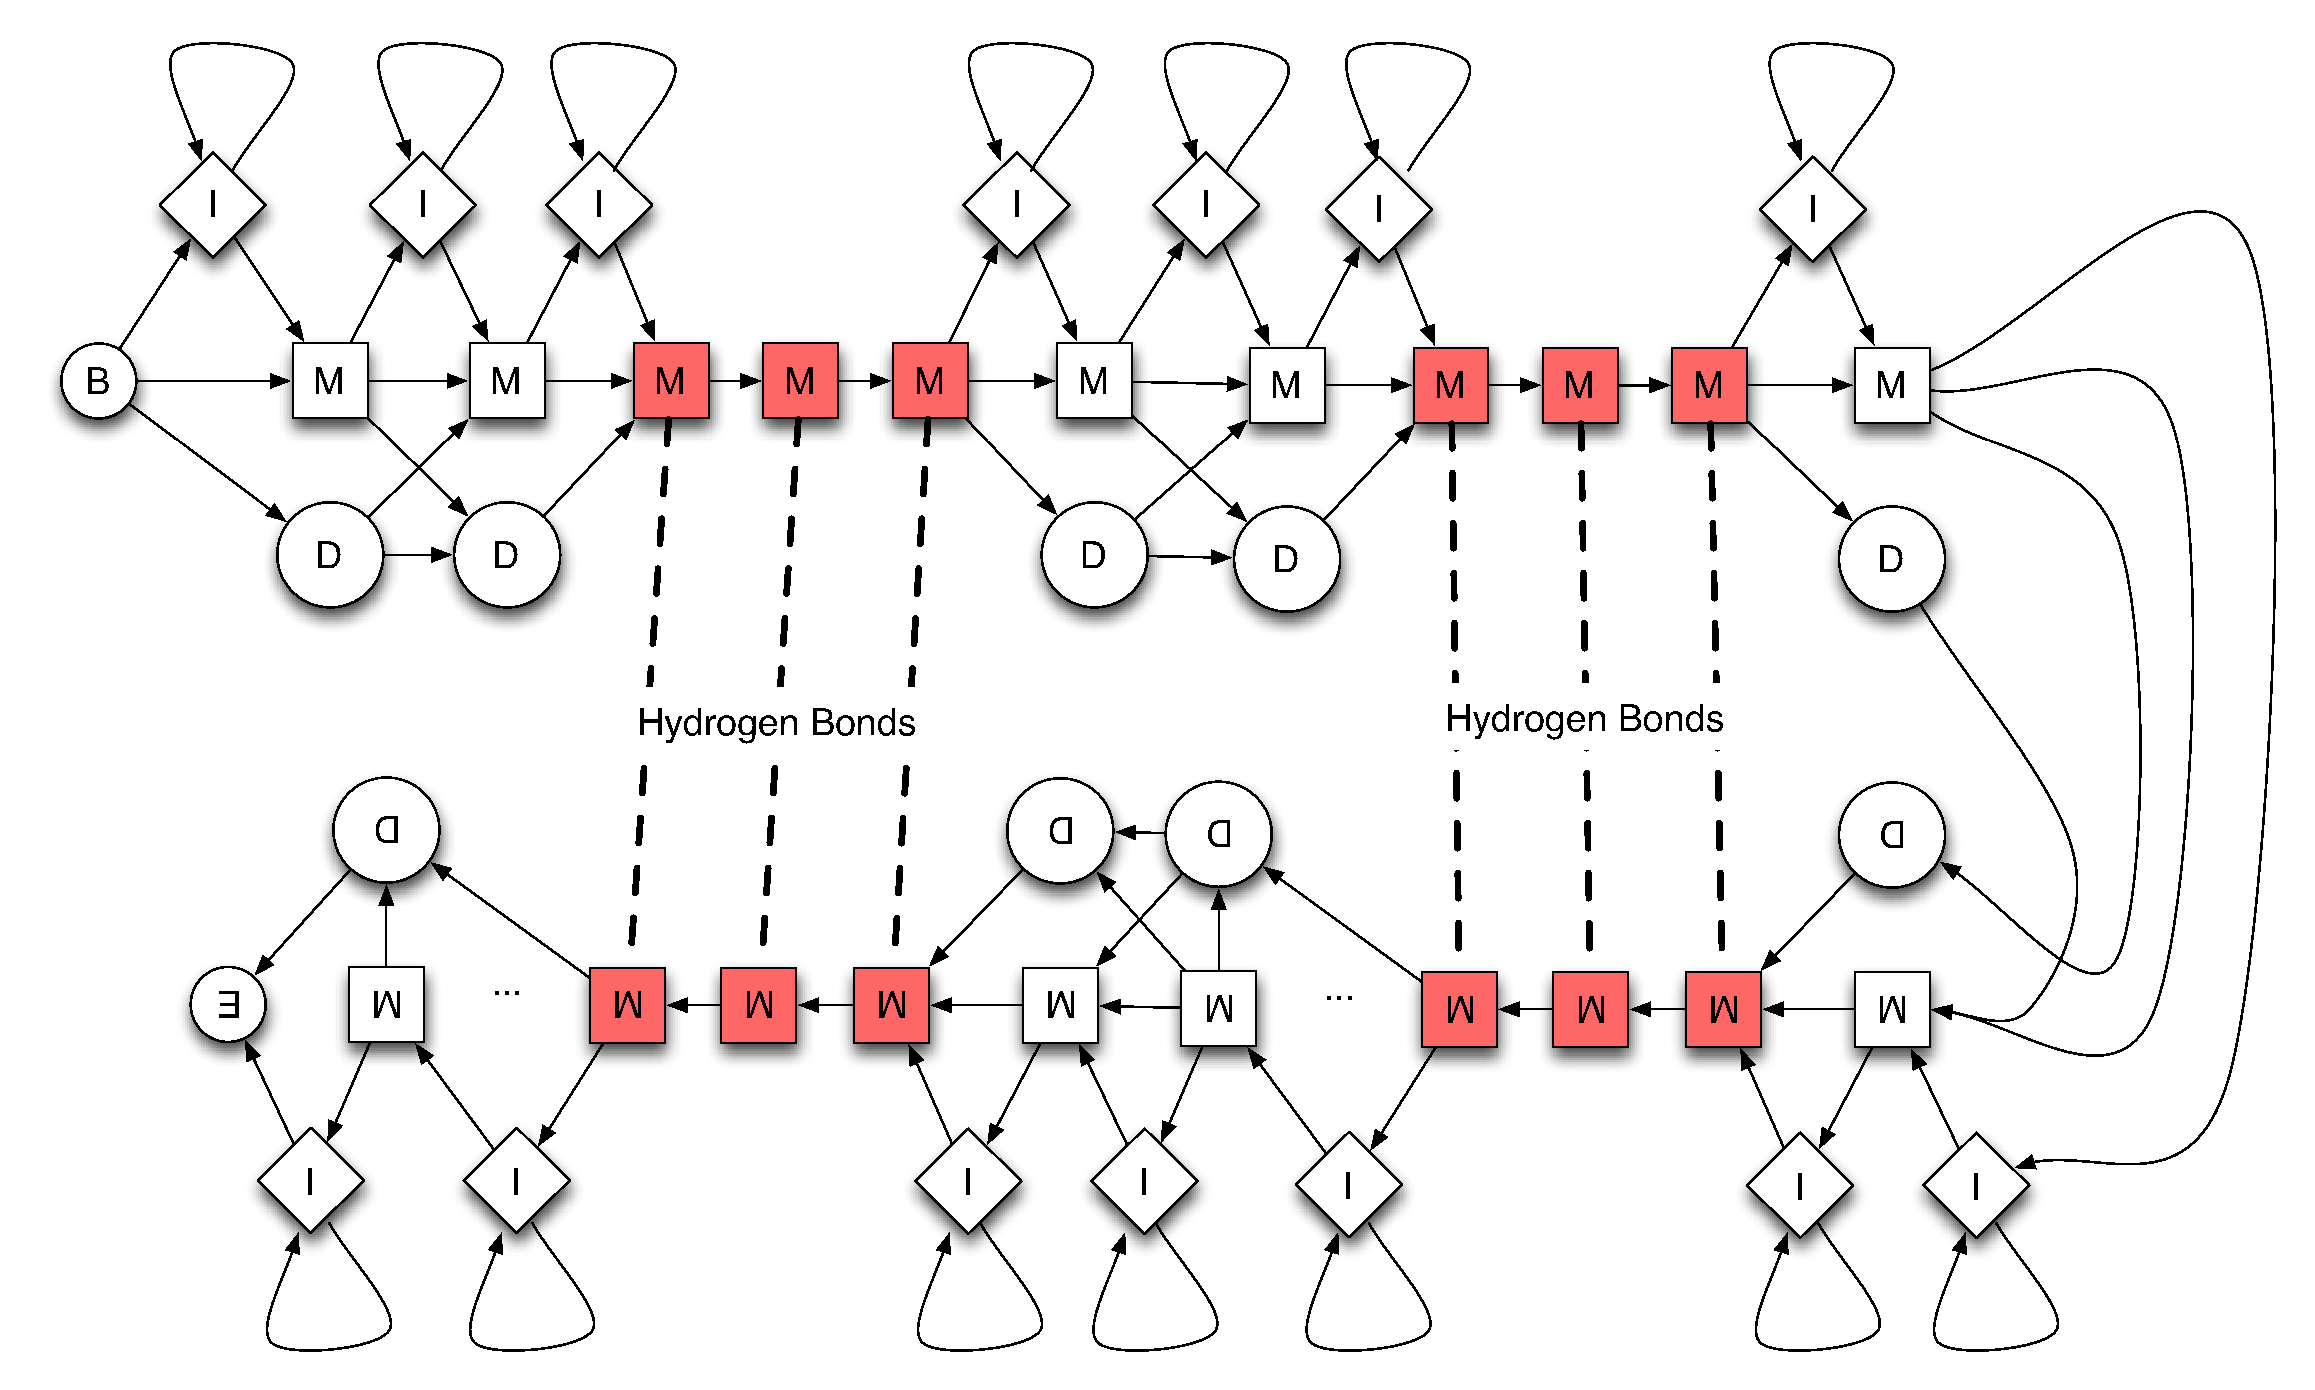
\includegraphics[width=8cm]{mrf_interleave_diagram.eps}} 
\fi
In this Markov random field,
each shaded node represents a beta-strand position.
Nodes connected by dashed edges are hydrogen-bonded.

\caption{A Markov random field with two beta-stand pairs}
\label{mrf} 
\end{figure}



MRFy treats the beta 
strands, which are build into the model,
 as ``beads'' which can be slid along the query sequence to determine
 a \emph{placement} of the beta strands.
A~placement's probability is computed
based on observed frequencies of paired amino acids in 
hydrogen-bonded beta strands~\cite{Cowen:2002p588}.
Given a placement, the maximum likelihood of any subsequence that appears
\emph{between} two beta strands can be computed exactly and
efficiently using Viterbi's algorithm.
(The result of the exact computation is a probability that is
\emph{conditioned} on the placement.)
MRFy searches for placements stochastically,
trying to maximize the product of these probabilities.
We~are exploring several
heuristics: random-mutation hill climbing, simulated 
annealing, multistart simulated annealing, and a genetic algorithm.
Our~exploration of these heuristics relies on higher-order functions.

These various search heuristics differ in how they approach four subproblems:
how they \textit{initialize} the search with a starting guess or guesses;
how they \textit{mutate} a solution into a new one; how they decide whether
to \textit{accept} a solution over a previous one; how they decide when to
\textit{terminate} the search.
For example, random-mutation hill climbing only accepts better guesses,
while simulated annealing sometimes accepts worse guesses; a genetic algorithm
combines ``parent'' guesses in its mutate function, while random-mutation
hill climbing simply permutes a guess into a new one.

\emph{[In scope: Parameters, [BetaStrand], QuerySequence]}

1. Start with [PLacement]
2. At significant expense, any Placement can be assigned a Score


 terminate determines when to finally stop the search. Examples might
 be running for a predetermined number of generations, or stopping
 when we've gone N generations without achieving more than E
 improvement in score


We represent these various search heuristics as a \texttt{SearchStrategy}:
%%%%%%%%%%%%%%%%%%%%%%%%%%%%%%%%%%%%%%%%%%%%%%%%%%%%%%%%

\smallverbatiminput{strategy}

This \texttt{SearchStrategy} is passed (as part of \texttt{SearchParameters})
to our generic search function:
%%%%%%%%%%%%%%%%%%%%%%%%%%%%%%%%%%%%%%%%%%%%%%%%%%%%%%%%

\smallverbatiminput{search}

As one of the parameters to the top-level \texttt{search} function,
we provide a \texttt{SearchStrategy} data type, which we use to 
define specific search techniques.
We require a \texttt{SearchStrategy} to 
define four functions: \texttt{mutate}, \texttt{accept}, \texttt{terminate}, 
and \texttt{initialize}; we use the Haskell module system to allow sharing of 
some of these functions between different search strategies.
For example, both 
\textit{random mutation hill climb} and \textit{simulated annealing} use the 
same initialize and mutate functions, but very different accept functions.
In 
all, we implemented four search strategies: \textit{random mutation hill 
climb}, \textit{simulated annealing}, \textit{multistart simulated annealing}, 
and \textit{genetic algorithm}.
We found the implementation of the search 
function and search strategies to be pleasant, and the resulting code to be 
simple and elegant.
In an imperative language with object orientation like Ruby 
or Python, we likely would have used a class hierarchy to accomplish this.
We 
feel that this would have required more code, because object orientation is 
meant for encapsulating data as well as functions on those data; here we only 
wanted to encapsulate functions, as the data did not change.


We note that \texttt{seed} in \texttt{search} comes from a monadic random 
number generator in Main, but we wished for search itself to be pure at this 
level.
One advantage is that this allows for testing of the \texttt{search} 
function with no randomness at all: if we pass in a known number as the seed, 
behavior is entirely deterministic.



In MRFy, the Viterbi function is called several times (once for each 
non-beta-strand region) for each search generation.
Furthermore, in a 
population-based search such as \textit{multistart simulated annealing}, the 
scoring function (which itself calls Viterbi) is called many times per 
generation.
Beyond traditional profiling, we found parallelization to be an 
obvious way to improve runtime performance.
We found this to be trivial thanks 
to the \texttt{Control.Parallel} library.
We pass the Viterbi function to a map over all 
non-beta-strand regions of the model and query sequence, and these regions are 
independent of one another.
Similarly, we pass the scoring function to a map 
over the population of potential solutions, which are also independent.
We 
merely substituted \texttt{parmap rseq} for map.
MRFy now efficiently uses all six 
cores on an AMD workstation for a non-population-based simulated annealing 
search, and all forty-eight cores on a compute server for population-based 
searches.




Despite the beauty of some of the code we were able to write, we found several 
instances where the easiest path seemed to be to write ugly code.
The first of 
these relates to the otherwise elegant Viterbi function.
Our stochastic search 
approach calls the Viterbi function a tremendous number of times, and most of 
the program's runtime is spent in this function.
However, the Viterbi algorithm 
retains not just a score (the probability of the sequence given a state path) 
but also the state path itself.
We implemented this state path as a list of 
\texttt{Int}, and every step in the recursion conses a new element onto the 
list.
However, at each step of the stochastic search, we discard the state 
path; we are searching to optimize score only.
We only need the state path at 
the termination of the search, when we wish the program to output an alignment 
of the query sequence to the Markov random field model.
We found that 
optimizing the Viterbi function by removing this state path entirely improved 
runtime performance by nearly 50\%.
However, we still needed the Viterbi 
function to provide a state path when we called it after search finally 
terminated.
Thus, we wondered how to implement the Viterbi function so that a 
state path was optional.

In order to determine if this optimization was even worthwhile, we first wrote 
a quick and dirty approach that is shameful in any language, but easy: we 
duplicated code.
We copied \texttt{viterbi} to produce a \texttt{viterbiF} 
which did not retain state path.
Next, however, we wondered how to avoid code 
duplication.
Clearly, littering the code with conditionals would produce code 
that was ugly as well as less efficient.
We knew how we would solve this 
problem in other languages; we would have used macros in Lisp, or 
metaprogramming via \texttt{eval} in Ruby, to produce two versions of the 
function from one prototype.
We struggled, however, to solve this problem 
idiomatically in Haskell.

Rather than attempt to use \texttt{TemplateHaskell} to generate two versions of 
the Viterbi function, we wrote a higher-order function type 
\lstinline!type ScorePathCons a = a -> [a] -> [a]! and two functions conforming to that type:
\begin{smallverbatim}
consPath :: ScorePathCons a
consPath x xs = x:xs

consNoPath :: ScorePathCons a
consNoPath _ _ = []
\end{smallverbatim}

Then, depending on whether \texttt{viterbi} was called with \texttt{consPath} 
or \texttt{consNoPath} as a parameter, the path would or would not be 
allocated.
We found this higher-order function approach to be simple in code 
and in concept, and it imposes negligible run-time overhead as compared to 
having two distinct functions.

\subsection{Awkward Haskell}

Another source of ugliness resulted from adding cost-center annotations when we 
wished to profile our code.
GHC will happily add cost centers to top-level 
functions, but much of our program relies on sub-functions.
We found that 
manually adding \texttt{\{-SCC -\}} annotations to dozens of guard clauses and 
sub-functions harmed the readability of our program, such that we felt 
compelled to remove all such annotations as soon as we could.
In our prior 
experience with profiling tools such as kcachegrind, simply compiling with 
debug symbols -- rather than manually annotating many lines of code -- allowed 
the profiling tools to provide us enough information.
Without these 
annotations, both call-site and allocation profiles are relatively useless in 
GHC.
Perhaps a compile-time flag that would auto-annotate every equation -- 
even if the resulting cost center is simply named with a line number -- would 
make this task easier.

The final source of ugliness in our code came from attempts at debugging 
run-time errors.
MRFy relies on a source of input data -- the paired beta 
strands in the Markov random field -- which is represented in an awkward manner 
by the original SMURF program, and which is outside our control.
Rather than 
represent beta strands directly, SMURF represents pairings of residues, leaving 
us to infer and reconstruct beta strands.
This task was difficult due to 
unclear invariants around overlapping, doubly-paired beta strands (and it would 
have been difficult in any programming language; the difficulty was one of 
representation).
However, the debugging tools in GHC caused us some 
difficulties in determining the sources of run-time errors.
We used 
\texttt{trace} extensively, but this style of ``\texttt{printf} debugging'' 
littered our code.
Being initially unaware of the backtrace feature of the GHC 
profiler, we wrote wrappers around \texttt{Vector.slice} and \texttt{Vector.!} 
which themselves called trace, which at least kept our ``\texttt{printf} 
debugging'' less cluttered.
Nonetheless, we struggled with these runtime errors 
due to an awkward representation, and wished for debugging tools such as we 
might find in gdb, which would allow us to examine the stack when a backtrace 
occurs.
 
 
\section{Our previous code base compared}

Our previous computational biology projects include an enhancement to a protein 
structural aligner that previously came from our group, Matt~\cite{Menke:2008wu}.

Matt's code base contains approximately 12,000 lines of C++ code, and relies on 
data structures such as mutable oct-trees, vectors, and arrays, with 
significant amounts of clever pointer arithmetic.
Our enhancement involved 
modifying Matt to incorporate sequence information along with the structural 
aligner.
While we initially estimated this would be a three-month project, it 
took most of a year because the mutable data structures were difficult to 
repurpose, and the pointer arithmetic was too clever for its own good: since 
invariants were not clear, nearly every change resulted in new segfaults.
One 
enhancement, partial alignments (essentially a cosmetic manipulation of the 
output, but requiring deep information about some of the data structures) was 
deemed infeasible.
We believe we could have completed a ground-up rewrite in 
Haskell, with most of the run-time performance, in fewer than nine months.


In general, the failure modes we encounter most in C++ programming are 
segmentation faults, memory errors (due to pointer arithmetic and uninitialized 
memory) and heap exhaustion.
In contrast, the failure modes we most commonly 
see in Haskell code are type-check failures, or at worst, runtime errors around 
bounds checking of arrays and vectors.
While bounds checking failures have 
proved difficult to debug, they are still less so than C++ memory errors.


Haskell makes it difficult to write code in haste, because Haskell militates 
towards careful type-checking and clearly thought-out function contracts.

Unlike dynamic languages such as Ruby, and unlike C++, Haskell punishes the 
programmer who attempts to write code quickly with the goal of later making it 
work correctly.
We have found MRFy to be easier to enhance and maintain than 
our existing C++ code bases.
Despite the learning curve of Haskell, we 
implemented most of MRFy in roughly three months of part-time work.

 
\section{State of the practice}

\subsection{Our group then}
Programmers generally avoid reimplementing algorithms, but there may be good reasons for doing so.
Although the HMMER software contains an mature C++ implementation of the Viterbi algorithm,
a previous member of our group implemented \textit{multidimensional} dynamic programming for SMURF
in haste, resulting in 12,000 lines of undocumented code (including one function of 700 lines).
Though we are using the same Viterbi algorithm HMMER implements, we chose to reimplement it because
we wished to explore the design space of stochastic search techniques using higher order functions
in Haskell.
We found that reimplementing the Viterbi algorithm in Haskell was easy and pleasant.
In contrast, the programming effort to transform SMURF into SMURFLite, a minor evolution, required
several months of research to simply understand the SMURF codebase.

A set of enhancements to another large C++ implementation, the Matt~\cite{Menke:2008wu} structural
aligner, required nearly a year of programming due to complex mutable data structures being 
hard to repurpose.
In fact, we deemed one enhancement infeasible.
Our experience working with these C++ codebases largely involved the failure modes of
segmentation faults, memory errors, and heap exhaustion.

\subsection{Our group now}
Implementing MRFy in Haskell allowed us great flexibility to explore the space of stochastic search
techniques, initial guess heuristics, and search termination.
Higher order functions militate towards more flexibility, so that adding several planned features 
to MRFy should be easy.
The first functioning version of MRFy took roughly three months of part-time work.
The Haskell failure modes we have experienced have largely been typecheck errors; at the worst,
we have seen runtime errors around bounds checking of arrays and vectors, though we wanted
better debugging tools for these runtime errors.

\subsection{Computational biology at large}
There exists some excellent software in the computational biology community, though little of it
has been written in Haskell.
The training component of MRFy was modified from that of HMMER, and working with the HMMER
codebase was relatively pleasant, as data structures and their mutators are well documented.
BioHaskell exists (and we use \texttt{Bio.Sequence.Fasta} as a parser) but is not nearly as
complete as BioPython or BioRuby, which are heavily used in the community.
We hope that BioHaskell and other tools for computational biology in Haskell continue to mature.
\section{What we think about it}

\subsection{Our Background}

\remark{I moved this section from the Intro as per NR's suggestion. ---AG}
All three authors are members of the Tufts University Department of Computer
Science.
Noah Daniels has taken a graduate seminar in advanced functional
programming, which included some Haskell, and spent ten years in industry as a
professional programmer in languages such as Ruby, C, and C++.
Andrew Gallant has taken a programming languages course heavily focused on 
functional programming, but with no Haskell.
Norman Ramsey is the local expert, but he wrote no code for this project.

\subsection{Barriers}
\remark{I feel like a lot of this is a summary of some of the problems we've
  discussed previously in the paper. Is that okay? A summary may be worth it. 
---AG}

As inexperienced functional programmers developing a complex piece of
software in Haskell, we encountered some barriers.
The first of these was profiling with GHC.
We previously mentioned that profiling with GHC required annotating
cost centers by hand, producing ugly code.
Beyond that, we also found it very difficult to profile code at all.
In particular, profiling required that all installed libraries be re-compiled
with profiling support,which was a process that we could not replicate
consistently.

Another barrier we faced was how to test our code using QuickCheck.
Indeed, the barrier was so formidable in our case that we still have not been 
able to use it.
The problems we faced specifically were two-fold: How do we start testing
a complex module? How can we use QuickCheck to generate random inputs with 
complex constraints? 
We wished to test invariants around beta-strand placement 
(potential solutions in our stochastic search), but found the QuickCheck generator
to be difficult to write.

Finally, one last barrier we faced was debugging runtime errors.
Runtime errors in the form of out-of-bounds indexing were particularly 
difficult to track down because they were not accompanied by a stack trace.
(While profiling with GHC could help remedy this, profiling was itself a 
barrier, as previously mentioned.)
We had to resort to polluting our code with calls to the \texttt{trace} function 
in order to track down where the out-of-bounds errors were occurring.

% - profiling 
% - debugging 
 % [ talk about profiling and debugging problems where?] 
% [ something about quickcheck: how do we know when we have enough QC props? How do we start testing a complex module? ] 

\subsection{What you must know to succeed}
If others would like to follow in our footsteps, there are a few
things we believe one must know in order to succeed.
Firstly, some experience with functional programming concepts is a necessity. 
Specifically, coming from an imperative background, we found transforming input data 
from the HMMER file format without the ability to mutate state was difficult.
In contrast, writing ``pure math'' like the Viterbi algorithm felt easier
and more natural than it would have been in C++.

Secondly, identifying existing tools and libraries from Hackage that are mature 
is also important.
We found that some packages that could have been immensely useful---like one 
that provides backtraces---were either not maintained or contained bugs.
Some other packages like Pads were functional but immature, which resulted in 
additional code to work around the parts of Pads that had not been implemented 
yet. 
In contrast, other packages such as \texttt{Data.Memocombinators} were
useful and mature.

Finally, a ``local expert'' or someone available to talk to with functional 
programming expertise, can make the transition to a language like Haskell 
easier.
We don't believe a local expert is absolutely necessary, but answers 
specifically related to functional programming idioms were easier to find when 
a local expert was available.


\subsection{Evaluation}
\remark{I think we need more in this section. ---AG}
In hindsight, we feel that there are several key facets of our project in 
Haskell that deserve evaluation.
Firstly, we found that existing tools and libraries were plentiful and 
typically helped us greatly.
In particular, \texttt{Data.Memocombinators} made dynamic 
programming with Viterbi exquisitely simple and elegant.
\texttt{Control.Parallel.Strategies} also made the parallelization of Viterbi trivial.
Most of the tools we used came straight from Hackage, and although 
documentation of some form was almost always present, it was sometimes 
difficult to tell if a particular tool was right for us.
In particular, parts of the documentation were inaccessible to us as beginning 
functional programmers.
Documentation that was accessible to us typically contained straight-forward 
examples showing how to use that particular tool or library.

Another component worthy of evaluation is the debugging process.
Debugging in Haskell often takes the form of fixing type errors; which we think 
is a great thing.
However, in the case where debugging extends into runtime behavior, we couldn't 
find any clearly defined approach to effective debugging.
Stack traces are available via profiling, but this was difficult to find and 
as we mentioned, profiling had its own barriers.

Finally, we believe that we could have achieved a better division of modules in 
our project, but that conflicted with one our goals: to get publishable results
quickly. Despite being hasty programmers, we were still able to produce code 
that is easy to understand and easily extensible. Namely, in our experience, 
hasty Haskell code beats hasty code in a language like C or C++.

In summary, with Haskell, we didn't have to master a completely different 
design and development style but we did have to wrap our heads around 
functional programming.\remark{Andrew, look at the comments below this
part of the manuscript. See what you can do with them.}


% - What does the local expert do? Do you have to have one? 
%  
% - To the FP community: Those who want us to abandon our old tools for debugging imperative code have not provided a clear path to follow (both intellectually, and via software tools). 
%  
% - No obvious body of knowledge on code improvement. 
%  
% - The ecosystem contains tools that look promising and work great: Data.Memocombinators, Quickcheck, Parallel Strategies. 
% How to tell what's good? How did we discover what's good? 
% - Profiler can produce backtraces, but this was hard to discover. 

% \appendix
% \section{Appendix Title}
% 
% This is the text of the appendix, if you need one.

\acks

We thank Lenore Cowen, Kathleen Fisher, Benjamin Hescott, Bradford Larsen, and Nathan Ricci.


\bibliographystyle{plainnat}

% The bibliography should be embedded for final submission.

\bibliography{mrfy_experience_report}


\vfill

\begingroup
\advance\leftskip by 0pt plus 10em
\emph{The Haskell wave passes, and if you slide off the crest, you
drown.}
\endgroup




\end{document}
